\chapter{Validation/Case studies}

The created tools and platform are now functional for testing problems, however they have not yet been tested in real-world scenarios. They have to be validated with real case studies in the areas of biotechnology and health where the application of these tools is relevant.

\section{The Datasets}

In total, 3 datasets were used as case studies and Table~\ref{tab:case_studies} provides an overview of them. The last column contains the dataset size with the number of positive and negative labels.

\begin{table}[ht]
	\caption{Case studies.}
	\label{tab:case_studies}
    \centering
    \begin{tabular}{lp{2cm}p{3.5cm}p{5.5cm}l}
    	\toprule
    	\textbf{Year} & \textbf{Authors} & \textbf{Title} & \textbf{Focus} & \textbf{Size}\\\midrule
    	
    	2005 & \citeauthor{Pokholok2005Genome-wideYeast} & Genome-wide map of nucleosome acetylation and methylation in yeast~\cite{Pokholok2005Genome-wideYeast} & \gls{DNA} sequences wrapping around histone proteins & 7667/7296\\\midrule
    	
        2018 & \citeauthor{Zou2018AGenomics} & A primer on deep learning in genomics~\cite{Zou2018AGenomics} & Discovery of transcription-factor binding sites in \gls{DNA}. & 987/1013\\\midrule
        
        2020 & \citeauthor{Zhang2020DeepHE:Learning} & DeepHE~\cite{Zhang2020DeepHE:Learning} & Predicting human essential genes based on deep learning. & 2010/11900\\
        
    	\bottomrule
    \end{tabular}
\end{table}

The first dataset used in this study, as well as in a previous work in the literature~\cite{Nguyen2016DNANetwork}, is one of the datasets published by~\citeauthor{Pokholok2005Genome-wideYeast}~\cite{Pokholok2005Genome-wideYeast}. These datasets are about \gls{DNA} sequences wrapping around histone proteins. It is a method for storing and packing lengthy \gls{DNA} sequences within the nucleus of a cell. The chosen dataset contains histones of type H3, with 7667 positive labels and 7298 negative labels and sequences with length 500. \citeauthor{Nguyen2016DNANetwork}~\cite{Nguyen2016DNANetwork} achieved 89\% accuracy in the H3 dataset in their work.

The second dataset used was derived from a study of~\citeauthor{Zou2018AGenomics}~\cite{Zou2018AGenomics}. The authors addressed an important problem in functional genomics, which is the discovery of transcription-factor binding sites in \gls{DNA}. They created a neural network capable of discovering \gls{DNA} binding motifs based on the results of a test that evaluates whether a longer \gls{DNA} sequence binds to the protein or not. The dataset has 2000 \gls{DNA} sequences of length 50, with 987 positive labels and 1013 negative labels. According to the experiments, the model achieved 98\% accuracy on the testing data.

The third and last dataset used in this study was also used in a research paper from~\citeauthor{Zhang2020DeepHE:Learning}. The authors tackled the issue that the majority of essential gene prediction approaches based on \gls{ML} lack the necessary ability to handle the unbalanced learning problem that is inherent in the challenge, which may be one reason impacting their performance. By combining features from sequencing data and protein-protein interaction network, the authors proposed a \gls{DL}-based approach, \textit{DeepHE}, to predict human essential genes. According to the experiment results, \textit{DeepHE} outperformed \gls{ML} models, such as \gls{SVM}, Naive Bayes, \gls{RF}, and Adaboost, achieving results of 90\% accuracy on the testing data. 

\section{Data Collection and Transformation}

Both the first and second datasets were easily accessible. Each article included a link to the accompanying \textit{CSV} file containing the sequences and their labels and no further data cleaning was required. 

The third dataset was not as easily accessible. Instead of providing a \textit{CSV} file, the authors specified the names of the databases from which they got the data. They built the essential gene dataset from the DEG database~\cite{Luo2014DEGElements}, and obtained the non-essential gene sequences from Ensembl database~\cite{Ruffier2017EnsemblAnnotation}. The DEG database contained 16 different human essential genes datasets, and 8256 human genes are identified as essential in at least one of the 16 datasets. However, the authors assumed that about 10\% human genes might be essential genes, and decided to build the essential gene dataset with genes contained at least in 5 datasets, resulting in 2024 sequences.

Then, for the non-essential gene dataset, the authors only stated that they obtained the sequences from Ensembl. However, the Ensembl database contains many different queries and options, and the authors did not specify which ones they used. This lack of information made it difficult to obtain the exact same dataset as the used on the paper. The only provided information is that they downloaded the dataset from Ensembl and if any of the 8256 annotated essential \textit{DEG} genes were present in the new dataset, they were deleted, resulting in 12697 sequences.

As expected, the results of attempting to replicate these steps for the positive and negative datasets were not the same to those in the study. Only 2010 sequences were retrieved for the positive dataset, while 14416 unique sequences were obtained for the negative dataset. The size of the positive dataset is comparable to that of the study, but the negative still had a relevant discrepancy. 

However, it is important to note that the sequences did not have the same length, unlike the two first datasets. Figures~\ref{fig:deg_length} and~\ref{fig:negative}  provide a visualization of the sequence's length distribution in each dataset.

\begin{figure}[htbp]
    \centering
    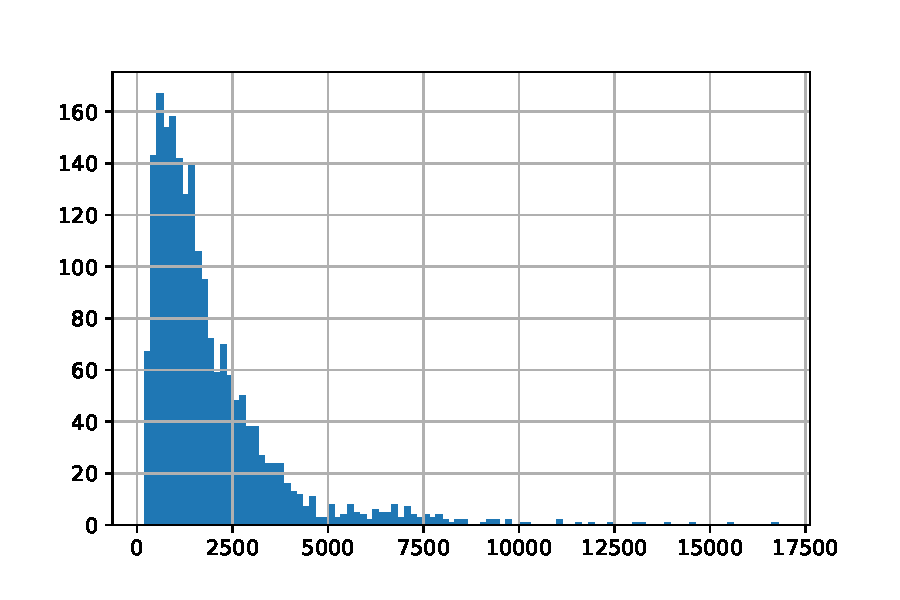
\includegraphics[width=0.7\linewidth]{positive}
    \caption{Sequence length and its occurrence in the positive dataset.}
    \label{fig:deg_length}
\end{figure}

\begin{figure}[htbp]
    \centering
    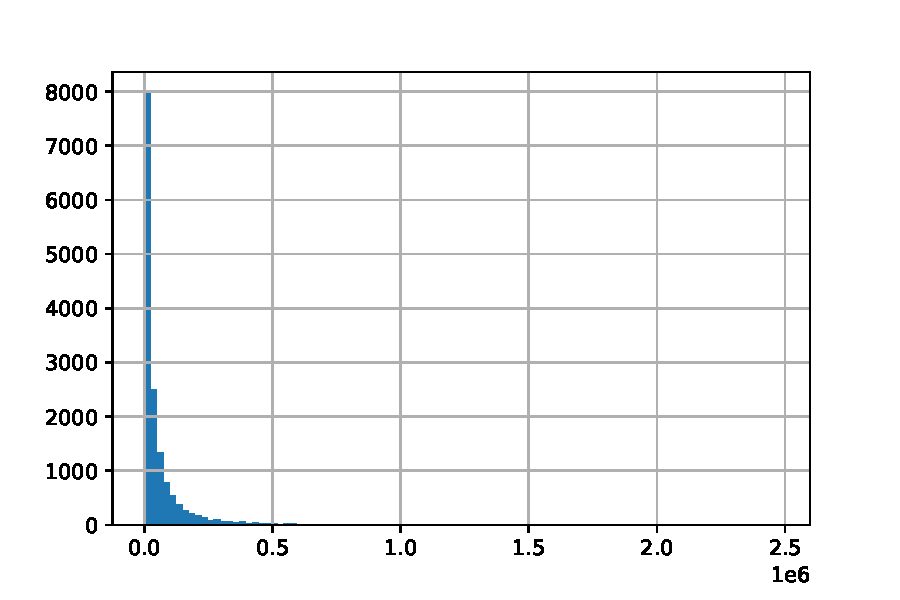
\includegraphics[width=0.7\linewidth]{negative}
    \caption{Sequence length and its occurrence in the negative dataset.}
    \label{fig:negative}
\end{figure}

A significant disparity in the length of the sequences was found in both datasets, especially in the negative one. The majority of the sequences have a length between 0 and 0.1e6. To remove some data noise, sequences that had length bigger than 0.1e6 were deleted, resulting in 11900 sequences (which is closer to the number of the negative dataset in the paper). Even though the lenghts of the positive dataset are not balanced either, no sequences were removed because the number of sequences was already very close to the paper's.

\begin{figure}[htbp]
    \centering
    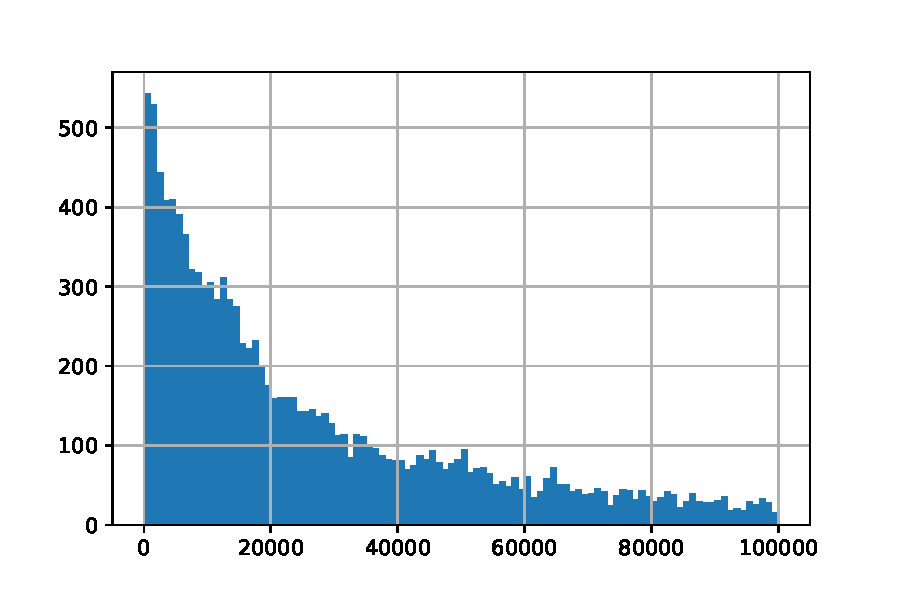
\includegraphics[width=0.7\linewidth]{negative_less_100k}
    \caption{Sequence length and its occurrence after removing sequences bigger than 0.1e6.}
    \label{fig:negative_less_100k}
\end{figure}

It is important to note that the final version of this dataset (2010 positives and 11900 negatives) is not balanced. Class weight were used to impose a heavier penalty when misclassifying an instance in the minority class, which is the class of important genes, to address the uneven data distributions between the two classes.

\section{Results and discussion of results}

To acquire the best possible results, it was necessary to test every combination of feature extraction - model - dataset. There are a total of four types of feature extraction techniques, twelve distinct models, and three datasets. This would need testing $4*12*3 = 144$ possibilities, however it is not necessary since some of these combinations are incompatible (some models only accept encodings and not descriptors and vice-versa). Therefore, 96 combinations were examined, and the results are shown below.

\begin{itemize}
    \item ('mlp', 'descriptor', 'primer')
    \item ('mlp\_half', 'descriptor', 'primer')
    \item ('cnn', 'one\_hot', 'primer')
    \item ('cnn', 'chemical', 'primer')
    \item ('cnn', 'kmer\_one\_hot', 'primer')
    \item ('cnn\_half', 'one\_hot', 'primer')
    \item ('cnn\_half', 'chemical', 'primer')
    \item ('cnn\_half', 'kmer\_one\_hot', 'primer')
    \item ('lstm', 'one\_hot', 'primer')
    \item ('lstm', 'chemical', 'primer')
    \item ('lstm', 'kmer\_one\_hot', 'primer')
    \item ('bi\_lstm', 'one\_hot', 'primer')
    \item ('bi\_lstm', 'chemical', 'primer')
    \item ('bi\_lstm', 'kmer\_one\_hot', 'primer')
    \item ('gru', 'one\_hot', 'primer')
    \item ('gru', 'chemical', 'primer')
    \item ('gru', 'kmer\_one\_hot', 'primer')
    \item ('bi\_gru', 'one\_hot', 'primer')
    \item ('bi\_gru', 'chemical', 'primer')
    \item ('bi\_gru', 'kmer\_one\_hot', 'primer')
    \item ('cnn\_lstm', 'one\_hot', 'primer')
    \item ('cnn\_lstm', 'chemical', 'primer')
    \item ('cnn\_lstm', 'kmer\_one\_hot', 'primer')
    \item ('cnn\_bi\_lstm', 'one\_hot', 'primer')
    \item ('cnn\_bi\_lstm', 'chemical', 'primer')
    \item ('cnn\_bi\_lstm', 'kmer\_one\_hot', 'primer')
    \item ('cnn\_gru', 'one\_hot', 'primer')
    \item ('cnn\_gru', 'chemical', 'primer')
    \item ('cnn\_gru', 'kmer\_one\_hot', 'primer')
    \item ('cnn\_bi\_gru', 'one\_hot', 'primer')
    \item ('cnn\_bi\_gru', 'chemical', 'primer')
    \item ('cnn\_bi\_gru', 'kmer\_one\_hot', 'primer')
    \item ('mlp', 'descriptor', 'h3')
    \item ('mlp\_half', 'descriptor', 'h3')
    \item ('cnn', 'one\_hot', 'h3')
    \item ('cnn', 'chemical', 'h3')
    \item ('cnn', 'kmer\_one\_hot', 'h3')
    \item ('cnn\_half', 'one\_hot', 'h3')
    \item ('cnn\_half', 'chemical', 'h3')
    \item ('cnn\_half', 'kmer\_one\_hot', 'h3')
    \item ('lstm', 'one\_hot', 'h3')
    \item ('lstm', 'chemical', 'h3')
    \item ('lstm', 'kmer\_one\_hot', 'h3')
    \item ('bi\_lstm', 'one\_hot', 'h3')
    \item ('bi\_lstm', 'chemical', 'h3')
    \item ('bi\_lstm', 'kmer\_one\_hot', 'h3')
    \item ('gru', 'one\_hot', 'h3')
    \item ('gru', 'chemical', 'h3')
    \item ('gru', 'kmer\_one\_hot', 'h3')
    \item ('bi\_gru', 'one\_hot', 'h3')
    \item ('bi\_gru', 'chemical', 'h3')
    \item ('bi\_gru', 'kmer\_one\_hot', 'h3')
    \item ('cnn\_lstm', 'one\_hot', 'h3')
    \item ('cnn\_lstm', 'chemical', 'h3')
    \item ('cnn\_lstm', 'kmer\_one\_hot', 'h3')
    \item ('cnn\_bi\_lstm', 'one\_hot', 'h3')
    \item ('cnn\_bi\_lstm', 'chemical', 'h3')
    \item ('cnn\_bi\_lstm', 'kmer\_one\_hot', 'h3')
    \item ('cnn\_gru', 'one\_hot', 'h3')
    \item ('cnn\_gru', 'chemical', 'h3')
    \item ('cnn\_gru', 'kmer\_one\_hot', 'h3')
    \item ('cnn\_bi\_gru', 'one\_hot', 'h3')
    \item ('cnn\_bi\_gru', 'chemical', 'h3')
    \item ('cnn\_bi\_gru', 'kmer\_one\_hot', 'h3')
    \item ('mlp', 'descriptor', 'essential\_genes')
    \item ('mlp\_half', 'descriptor', 'essential\_genes')
    \item ('cnn', 'one\_hot', 'essential\_genes')
    \item ('cnn', 'chemical', 'essential\_genes')
    \item ('cnn', 'kmer\_one\_hot', 'essential\_genes')
    \item ('cnn\_half', 'one\_hot', 'essential\_genes')
    \item ('cnn\_half', 'chemical', 'essential\_genes')
    \item ('cnn\_half', 'kmer\_one\_hot', 'essential\_genes')
    \item ('lstm', 'one\_hot', 'essential\_genes')
    \item ('lstm', 'chemical', 'essential\_genes')
    \item ('lstm', 'kmer\_one\_hot', 'essential\_genes')
    \item ('bi\_lstm', 'one\_hot', 'essential\_genes')
    \item ('bi\_lstm', 'chemical', 'essential\_genes')
    \item ('bi\_lstm', 'kmer\_one\_hot', 'essential\_genes')
    \item ('gru', 'one\_hot', 'essential\_genes')
    \item ('gru', 'chemical', 'essential\_genes')
    \item ('gru', 'kmer\_one\_hot', 'essential\_genes')
    \item ('bi\_gru', 'one\_hot', 'essential\_genes')
    \item ('bi\_gru', 'chemical', 'essential\_genes')
    \item ('bi\_gru', 'kmer\_one\_hot', 'essential\_genes')
    \item ('cnn\_lstm', 'one\_hot', 'essential\_genes')
    \item ('cnn\_lstm', 'chemical', 'essential\_genes')
    \item ('cnn\_lstm', 'kmer\_one\_hot', 'essential\_genes')
    \item ('cnn\_bi\_lstm', 'one\_hot', 'essential\_genes')
    \item ('cnn\_bi\_lstm', 'chemical', 'essential\_genes')
    \item ('cnn\_bi\_lstm', 'kmer\_one\_hot', 'essential\_genes')
    \item ('cnn\_gru', 'one\_hot', 'essential\_genes')
    \item ('cnn\_gru', 'chemical', 'essential\_genes')
    \item ('cnn\_gru', 'kmer\_one\_hot', 'essential\_genes')
    \item ('cnn\_bi\_gru', 'one\_hot', 'essential\_genes')
    \item ('cnn\_bi\_gru', 'chemical', 'essential\_genes')
    \item ('cnn\_bi\_gru', 'kmer\_one\_hot', 'essential\_genes')
\end{itemize}
